%%%%%%%%%%%%%%%%%%%%%%%%%%%%%%%%%%%%%%%%%%%%%%%%%%%%%%%%%%%%%%%
%
%     filename  = "Dissertation Index.tex",
%     version   = "Draft 1",
%     date      = "1/16/2013",
%     authors   = "Nicholas P. Nicoletti",
%     copyright = "Nicholas P. Nicoletti",
%     address   = "Department of Political Science,
%                  516 Park Hall,
%                  University at Buffalo,
%                  Buffalo, NY 14260,
%                  USA",
%     telephone = "(585) 752-5167",
%     email     = "npn@buffalo.edu",
%
%%%%%%%%%%%%%%%%%%%%%%%%%%%%%%%%%%%%%%%%%%%%%%%%%%%%%%%%%%%%%%%
%
% Change History:
%
% Draft Version 1.0 - No Changes.
%
%%%%%%%%%%%%%%%%%%%%%%%%%%%%%%%%%%%%%%%%%%%%%%%%%%%%%%%%%%%%%%%
%
% This is a template file to help get you started using the
% psuthesis.cls for theses and dissertations at Penn State
% University. You will, of course, need to put the
% psuthesis.cls file someplace that LaTeX will find it.
%
% We have set up a directory structure that we find to be clean
% and convenient. You can readjust it to suit your tastes. In
% fact, the structure used by our students is even a little
% more involved and commands are defined to point to the
% various directories.
%
% This document has been set up to be typeset using pdflatex.
% About the only thing you will need to change if typesetting
% using latex is the \DeclareGraphicsExtensions command.
%
% The psuthesis document class uses the same options as the
% book class. In addition, it requires that you have the
% ifthen, calc, setspace, and tocloft packages.
%
% The first additional option specifies the degree type. You
% can choose from:
%     Ph.D. using class option <phd>
%     M.S. using class option <ms>
%     M.Eng. using class option <meng>
%     M.A. using class option <ma>
%     B.S. using class option <bs>
%     B.A. using class option <ba>
%     Honors Baccalaureate using the option <honors>
%
% If you specify either ba or bs in addition to honors, it will
% just use the honors option and ignore the ba or bs option.
%
% The second additional option <inlinechaptertoc> determines
% the formatting of the Chapter entries in the Table of
% Contents. The default sets them as two-line entries (try it).
% If you want them as one-line entries, issue the
% inlinechaptertoc option.
%
% The class option ``honors'' should be used for theses
% submitted to the Schreyer Honors College. This option
% changes the formatting on the Title page so that the
% signatures appear on the Title page. Be sure and comment
% out the command \psusigpage when using this option since it
% is not needed and it messes up the vertical spacing on the
% Title page.
%
% The class option ``honorsdepthead'' adds the signature of the
% department head on the Title page for those baccalaureate
% theses that require this.
%
% The class option ``secondthesissupervisor'' should be used
% for baccalaureate honors degrees if you have a second
% Thesis Supervisor.
%
% The vita is only included with the phd option and it is
% placed at the end of the thesis. The permissions page is only
% included with the ms, meng, and ma options.
%%%%%%%%%%%%%%%%%%%%%%%%%%%%%%%%%%%%%%%%%%%%%%%%%%%%%%%%%%%%%%%
% Only one of the following lines should be used at a time.
\documentclass[phd,12pt]{psuthesis}
%\documentclass[draft,phd,inlinechaptertoc]{psuthesis}
%\documentclass[draft,ms]{psuthesis}
%\documentclass[draft,honorsdepthead,honors]{psuthesis}
%\documentclass[draft,honors]{psuthesis}
%\documentclass[draft,secondthesissupervisor,honors]{psuthesis}
%\documentclass[draft,bs]{psuthesis}


%%%%%%%%%%%%%%%%%%%%%%%%%%%%
% Packages we like to use. %
%%%%%%%%%%%%%%%%%%%%%%%%%%%%
\usepackage{amsmath}
\usepackage{amssymb}
\usepackage{amsthm}
\usepackage{exscale}
\usepackage[mathscr]{eucal}
\usepackage{bm}
\usepackage{eqlist} % Makes for a nice list of symbols.
\usepackage[final]{graphicx}
\usepackage[dvipsnames]{color}
\DeclareGraphicsExtensions{.pdf, .jpg, .png}
\usepackage{natbib}
\usepackage{har2nat}
\usepackage{verbatim}
\usepackage{url}
\usepackage{longtable}
\usepackage{mathpazo}
\usepackage{pstricks}
\usepackage{sgamevar}
\usepackage{egameps}
\def\citeapos#1{\citeauthor{#1}'s \citeyear{#1}}
\newenvironment{my_enumerate}
{\begin{enumerate}
  \setlength{\itemsep}{1pt}
  \setlength{\parskip}{0pt}
  \setlength{\parsep}{0pt}}{\end{enumerate}}
\newenvironment{my_itemize}
{\begin{itemize}
  \setlength{\itemsep}{1pt}
  \setlength{\parskip}{0pt}
  \setlength{\parsep}{0pt}}{\end{itemize}}


%%%%%%%%%%%%%%%%%%%%%%%%
% Setting for fncychap %
%%%%%%%%%%%%%%%%%%%%%%%%
% Comment out or remove the next two lines and you will get
% the standard LaTeX chapter titles. We like these A LOT
% better.
\usepackage[Lenny]{fncychap}
\ChTitleVar{\Huge\sffamily\bfseries}


%%%%%%%%%%%%%%%%%%%%%%%%%%%%%%%
% Use of the hyperref package %
%%%%%%%%%%%%%%%%%%%%%%%%%%%%%%%
%
% This is optional and is included only for those students
% who want to use it.
%
% To use the hyperref package, uncomment the following line:
%\usepackage[colorlinks=true,urlcolor=purple,citecolor=green,linkcolor=blue]{hyperref}
%
% Note that you should also uncomment the following line:
%\renewcommand{\theHchapter}{\thepart.\thechapter}
%
% to work around some problem hyperref has with the fact
% the psuthesis class has unnumbered pages after which page
% counters are reset.


%%%%%%%%%%%%%%%%%%%%%%%%%%%%%%%%%%%%
% SPECIAL SYMBOLS AND NEW COMMANDS %
%%%%%%%%%%%%%%%%%%%%%%%%%%%%%%%%%%%%
% Place user-defined commands below.

\graphicspath{
{Chapter-2/Figures/}
{Chapter-3/Figures/}
{Chapter-4/Figures/}
}

\usepackage{xspace}
\usepackage{mfirstuc}
\usepackage{multirow}
\usepackage{subcaption}

\newcommand{\engine}{Emulation Engine}
\newcommand*{\eg}{e.g.\@\xspace}
\newcommand*{\ie}{i.e.\@\xspace}
\newcommand{\degree}{$^{\circ}$}

\usepackage{setspace}
\doublespacing



%%%%%%%%%%%%%%%%%%%%%%%%%%%%%%%%%%%%%%%%%
% Renewed Float Parameters              %
% (Makes floats fit better on the page) %
%%%%%%%%%%%%%%%%%%%%%%%%%%%%%%%%%%%%%%%%%
\renewcommand{\floatpagefraction}{0.85}
\renewcommand{\topfraction}      {0.85}
\renewcommand{\bottomfraction}   {0.85}
\renewcommand{\textfraction}     {0.15}

% ----------------------------------------------------------- %

%%%%%%%%%%%%%%%%
% FRONT-MATTER %
%%%%%%%%%%%%%%%%
% Title
\title{Differential Jet Production Cross Section Measurement in Z + Jet events from Proton - Proton Collisions at $\sqrt{s}$ = 13 TeV using the CMS detector at LHC}

% Author and Date of Degree Conferral or Defense
\author{Ashley Marie Parker}
% the degree will be conferred on this date
\degreedate{August 2019}
% year of your copyright. I have removed this from the cover page because UB's guidelines do not include it.
%\copyrightyear{2019}

% This is the document type. For example, this could also be:
%     Comprehensive Document
%     Thesis Proposal
\documenttype{Disseration}
%The department where you will be submitting the document%
\dept{Department of Physics}
% This will generally be The Graduate School, though you can
% put anything in here to suit your needs. This has also been removes from the cover page via the psuthesis.cls document because UB guidelines do not allow for it.
\submittedto{The Graduate School}


%%%%%%%%%%%%%%%%%%
% Signatory Page %
%%%%%%%%%%%%%%%%%%
% You can have up to 7 committee members, i.e., one advisor
% and up to 6 readers.
%
% Begin by specifying the number of readers.
\numberofreaders{3}


% Input reader information below. The optional argument, which
% comes first, goes on the second line before the name.
\advisor[Thesis Advisor, Chair of Committee]
        {Salvatore Rappoccio}
        {Professor of Physics}

\readerone[Committee Member]
          {Ia Iashvili}
          {Professor of  Physics}

\readertwo[Committee Member]
          {Ciaran Williams}
          {Professor of  Physics}




% Makes use of LaTeX's include facility. Add as many chapters
% and appendices as you like.
\includeonly{%
Chapter-1/chap1,%
Chapter-2/chap2,%
Chapter-3/chap3,%
Chapter-4/chap4,%
Chapter-5/chap5,%
%Appendix-A/main,%
%Appendix-B/main%
}

%%%%%%%%%%%%%%%%%
% THE BEGINNING %
%%%%%%%%%%%%%%%%%
\begin{document}

%%%%%%%%%%%%%%%%%%%%%%%%
% Preliminary Material %
%%%%%%%%%%%%%%%%%%%%%%%%
% This command is needed to properly set up the frontmatter.
\frontmatter

%%%%%%%%%%%%%%%%%%%%%%%%%%%%%%%%%%%%%%%%%%%%%%%%%%%%%%%%%%%%%%
% IMPORTANT
%
% The following commands allow you to include all the
% frontmatter in your thesis. If you don't need one or more of
% these items, you can comment it out. Most of these items are
% actually required by the Grad School -- see the Thesis Guide
% for details regarding what is and what is not required for
% your particular degree.
%%%%%%%%%%%%%%%%%%%%%%%%%%%%%%%%%%%%%%%%%%%%%%%%%%%%%%%%%%%%%%
% !!! DO NOT CHANGE THE SEQUENCE OF THESE ITEMS !!!
%%%%%%%%%%%%%%%%%%%%%%%%%%%%%%%%%%%%%%%%%%%%%%%%%%%%%%%%%%%%%%

% Generates the signature page. This is not bound with your
% thesis.
%\psusigpage

\pagestyle{plain}
\pagenumbering{roman}

% Generates the title page based on info you have provided
% above.
\psutitlepage

%Generates Copyright Page
\copyrightpage{SupplementaryMaterial/Copyright}

\newpage
% Generates the committee page -- this is bound with your
% thesis. If this is an baccalaureate honors thesis, then
% comment out this line.
% \psucommitteepage

% Generates the Epigraph/Dedication. The first argument should
% point to the file containing your Epigraph/Dedication and
% the second argument should be the title of this page.
%\thesisdedication{SupplementaryMaterial/Dedication}{Dedication}

% Generates the Acknowledgments. The argument should point to
% the file containing your Acknowledgments.
%\thesisacknowledgments{SupplementaryMaterial/Acknowledgments}

% Generates the Table of Contents
\thesistableofcontents

% Generates the List of Tables
\thesislistoftables

% Generates the List of Figures
\thesislistoffigures

% Generates the List of Symbols. The argument should point to
% the file containing your List of Symbols.
% \thesislistofsymbols{SupplementaryMaterial/ListOfSymbols}

% Generates the abstract. The argument should point to the
% file containing your abstract.
\thesisabstract{SupplementaryMaterial/Abstract}


\pagenumbering{arabic}

%%%%%%%%%%%%%%%%%%%%%%%%%%%%%%%%%%%%%%%%%%%%%%%%%%%%%%
% This command is needed to get the main part of the %
% document going.                                    %
%%%%%%%%%%%%%%%%%%%%%%%%%%%%%%%%%%%%%%%%%%%%%%%%%%%%%%
\thesismainmatter

%%%%%%%%%%%%%%%%%%%%%%%%%%%%%%%%%%%%%%%%%%%%%%%%%%
% This is an AMS-LaTeX command to allow breaking %
% of displayed equations across pages. Note the  %
% closing the "}" just before the bibliography.  %
%%%%%%%%%%%%%%%%%%%%%%%%%%%%%%%%%%%%%%%%%%%%%%%%%%
\allowdisplaybreaks{
%
%%%%%%%%%%%%%%%%%%%%%%
% THE ACTUAL CONTENT %
%%%%%%%%%%%%%%%%%%%%%%
% Chapters
\chapter{Theoretical Framework}%\label{ch1:intro}

%\vspace{-5pt}

%%\section{Motivation}\label{secMot:ch1}

%Within this dissertation, I provide a measurement of the differential jet cross section, as a function of the jet mass and transverse momentum, in events with a Z + Jet topology using data collected by CMS experiment at LHC. 


















%%%%%%%%%%%%%%%%%%%%%%%%%%%%%%%%%%%%%%%%%%%%%%%%%%%%%%
\section{The Standard Model}\label{secSM:ch1}

%"Theorists can be wrong; only nature is always right" - David Gross
"Fortunately, nature is as generous with its problems as Nobel with his fortune. The more we know, the more aware we are of what we know not."- David Gross \newline

The Standard Model, SM, of particle physics constitues humanity's latest attempt at describing our universe in a calculable way. The basic premise being, the entire universe is compised solely of; 6 types of quark and 6 types of lepton, which comprise matter, and the guage bosons, which mediate the 3 (this theory does not yet encompass gravitaion) fundamental forces; The strong and weak nuclear interactions and electromagnetism. 


Various attempts have been made to unify the fundamental forces under one theory, thusfar the electromagnetic and weak interactions have been united by electro-weak theory. 

The Standard electroweak model can be described $SU(2) x U(1)$ mathematically.

The  $SU(2) x U(1)$ guage group is a convolution ( $<- $That is not the right word...) of the special unitary symmetry group $SU(2)$ describing 3 mixed massive vector bosons, $W_{-}$ $W_{+}$ $Z_0$, carriers of the weak nuclear force and the unitary gauge group $U(1)$ , describing the lonely massless chargeless photon, of the electromagnetic interaction.

The standard model of the strong interaction is known as quatum chromodynamics, QCD, described by the special unitary group $(SU(3)_f)$, where the  flavours of quark are the physical manifestation of the symmetry group. This force is mediated by the 8 massless gluons which carry color charge, making QCD more complicated mathematically than QED.

The SM also contains a Higgs boson, an excitation of a scalar Higg's field, which gives rise to spantaneous symmetry breaking of the electroweak theory, providing the particles with mass, but I won't get into that. 

The quarks and leptons are arranged in generations according to their relative masses, as shown in Figure \ref{fig:SM}. The table also shows the spins of the particles, the leptons and quarks have half-integer spin, fermions, that obey the fermi exclusion principle, conversely the bosons have half integer spin and therefore obey bose-einstein statitics. Through the SM we interpret the observed hadronic particles, mesons ( baryons ) , as 2 quark (3 quark) bound states. The existence of spin $\frac{3}{2}$ baryons, which are symmetric bound states in space, spin and flavour and the need to obey Fermi-Dirac statistics, by maintaining total assymmetry of the wavefunction,implies there is another degree of freedom, called color, so that each quark is either red, green or blue. Granted only color singlet, containing either all 3 or 1 and it's anti color, states exist. Furthermore there exists a property of asymptotic freedom where the QCD coupling between quarks and gluons increases as they asymptotically approach one another. There exists a wealth of experiemental data to support the concept of asymptotic freedom despite the fact that rigorous mathematical proof of the exlusion of free quark and gluon states has yet to be acheived.


%image CMS:2014mna
% visuals/strong-coupling-cms


\begin{figure}[htb]
\centering
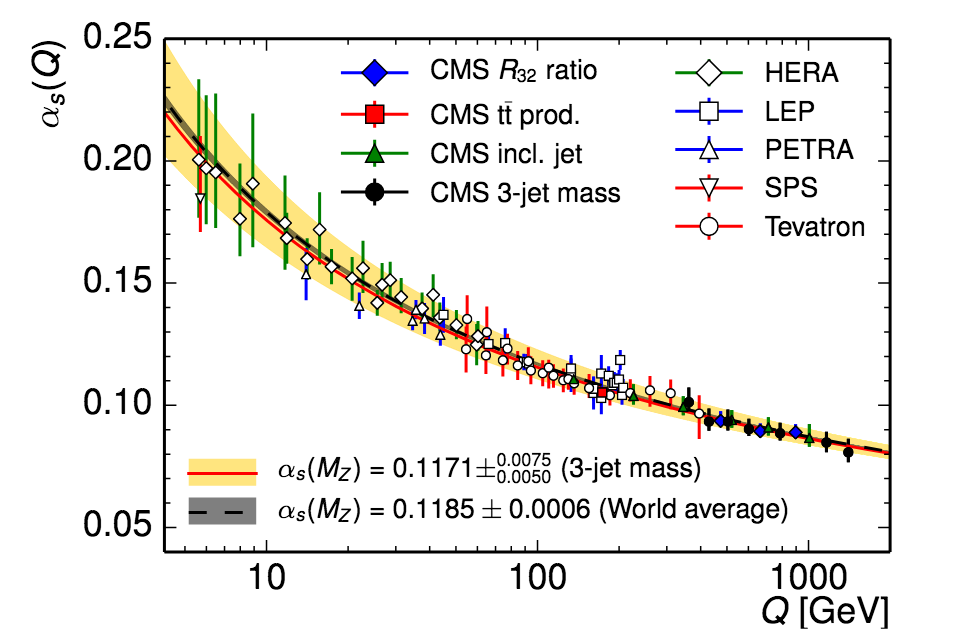
\includegraphics[width=1.0\textwidth]{visuals/strong-coupling-cms.png}
\caption{The running of the strong coupling constand as compiled by CMS including measurements from CMS and HERA among others~\cite{CMS:2014mna}.}
\label{fig:alphas}
\end{figure}







Assymptotic freedom is a useful property as it allows for perturbative calculations of QCD observables, this is discussed in section XXX.

% Symmetris imply conserved quantities, Neuther's Theorem

 Nuclei in ordinary matter are composed solely of $1^{st}$ generation particles, up and down quarks, bound by gluons. Neutral atoms contain an equal number of protons (composed of 2 up quarks and a down quark) and electrons, $1^{st}$ generation leptons. The main distinction between leptons and quarks, both fermions (particles of $\frac{1}{2}$ integer spin), being that leptons do not experience the color interaction $(SU(3)_f)$ like their quark friends. In each generation there is a quark with charge $Q = + \frac{2}{3}$ (up, charm, top) and another of charge $Q = - \frac{1}{3}$ (down, strange, bottom).



\begin{figure}[htb]
\centering
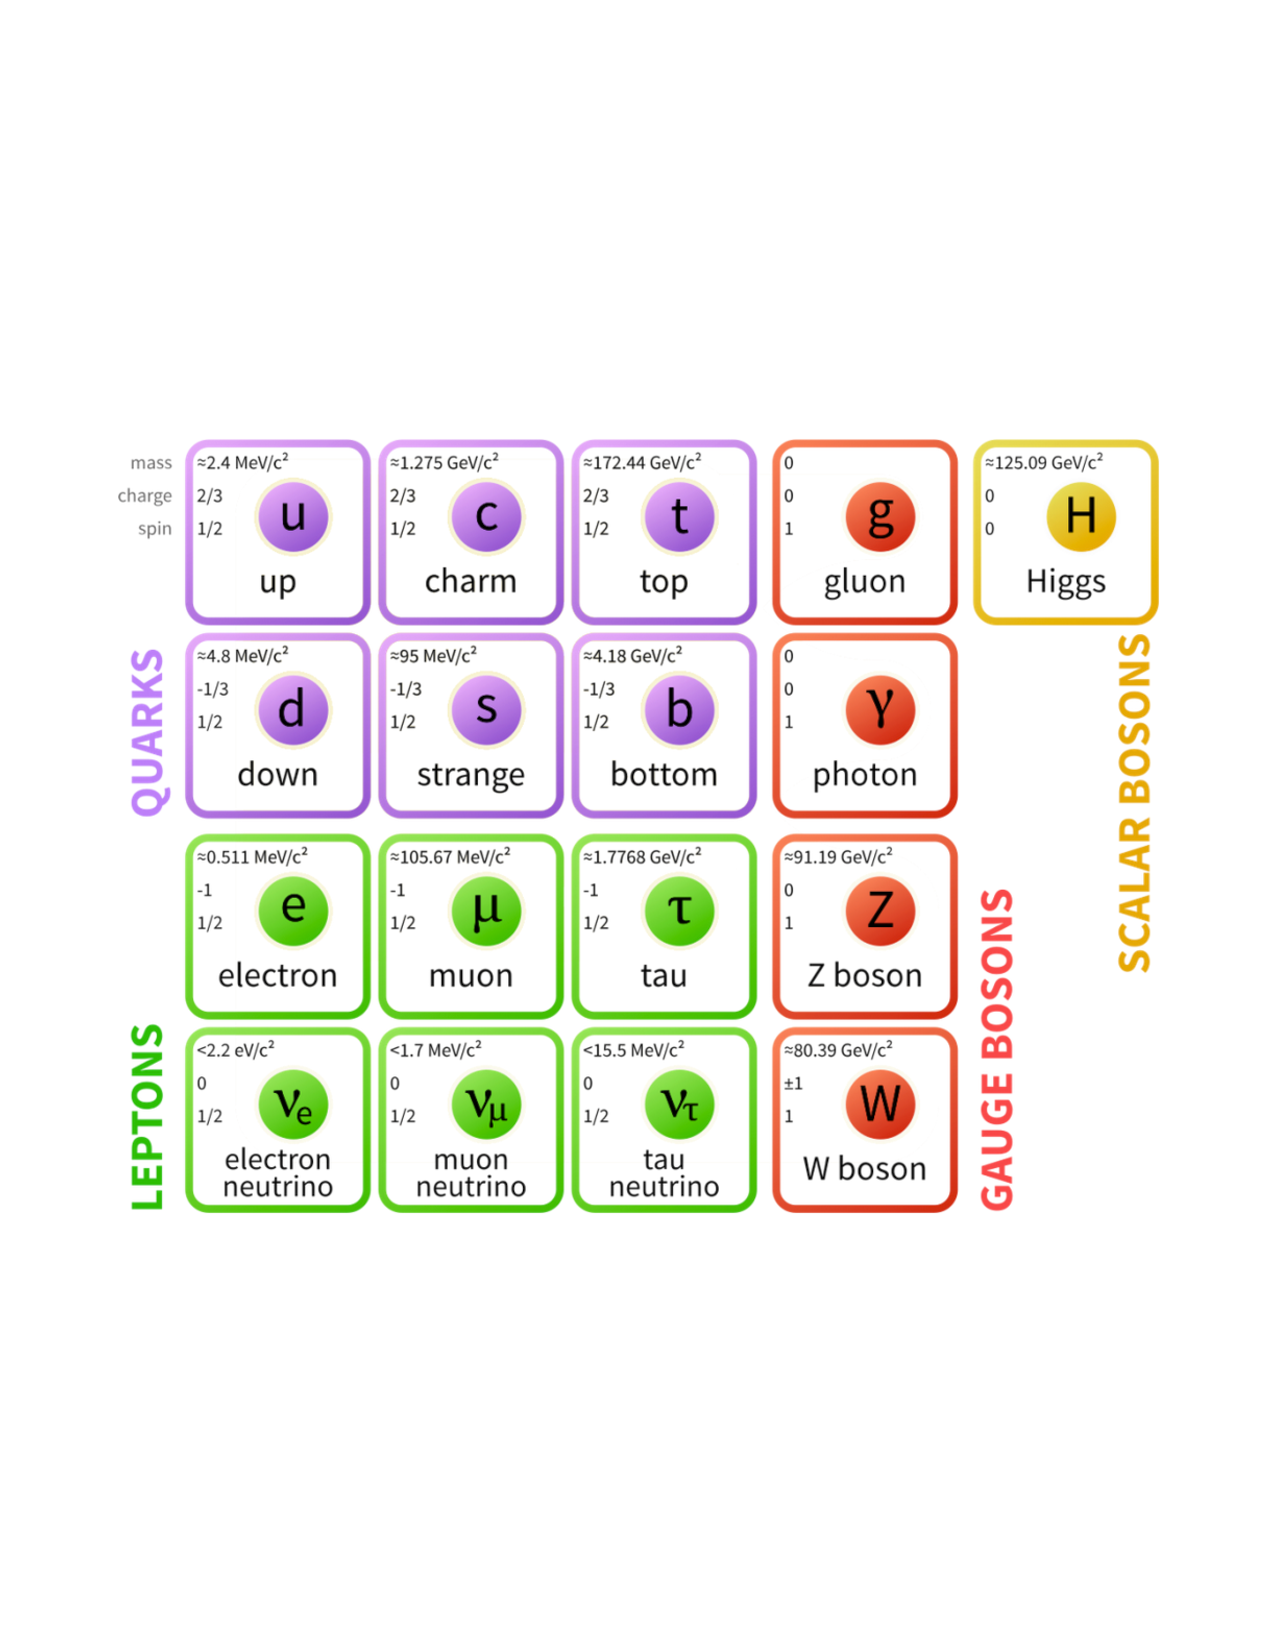
\includegraphics[width=1.0\textwidth]{smdiagram.pdf}
\caption{Fundamental particles of the Standard Model~\cite{modellinginvisible}.}
\label{fig:SM}
\end{figure}






\subsection{Quantum Chromodynamics}\label{secSM:ch1}


In order to emphasize the relevance to the measurement presented herein, the theory of Quantum Chromodynamics is discussed here from a kinematic (<- better word?) rather than Lagrangian perspective. This is useful as jet studies help probe QCD in the soft and collinear limits. 
% https://arxiv.org/pdf/1709.06195.pdf CITE THIS LECTURE
Jets are formed by the hadronization of quarks and gluons. In this thesis I present a measurement of a light quark enriched jet sample. 



Consider the simplest process that could produce a quark initiated jet, a quark of energy $E_q$  emitting a gluon of energy $E_g$. The probability that this will occur is a function of the gluon's energy fraction, $z$, and the emission angle , $\theta$  \cite{Larkoski:2017fip}.\newline


$z = \frac{E_g}{E_q + E_g}$\newline

$1 - cos \theta = \frac{m^2}{2 E_q E_g}$\newline

Then the probability of gluon emission from the quark is :


$P_q(z,cos \theta) dz d cos \theta = \frac{\alpha_s C_F}{\pi}  \frac{dz}{z} \frac{dcos \theta}{1 - cos \theta}  $\newline

It is useful to assume the small angle approximation, $\theta << 1$, giving:\newline


$P_q(z,\theta^2) dz d \theta^2 = \frac{\alpha_s C_F}{\pi}  \frac{dz}{z} \frac{d \theta^2}{ \theta^2}  $\newline

Notice that the probability of emission diverges for very soft (small z) or very collinear (small $\theta$) gluons. In the soft and collinear limits the probability can be interpretted as an expectation value for the number of soft/collinear gluons \cite{Larkoski:2017fip}.

It is elucidating to rewite the probability in terms of inverse logarithms in the and intruduce the "Lund Diagram" in order to visualize the uniform distribution of soft and collinear gluons in the $log \frac{1}{ \theta^2} , log\frac{1}{z} $ space.

The primary lund plane is shown in Figure XX ~\cite{Dreyer:2018nbf}
%image 

\begin{figure}[htb]
\centering
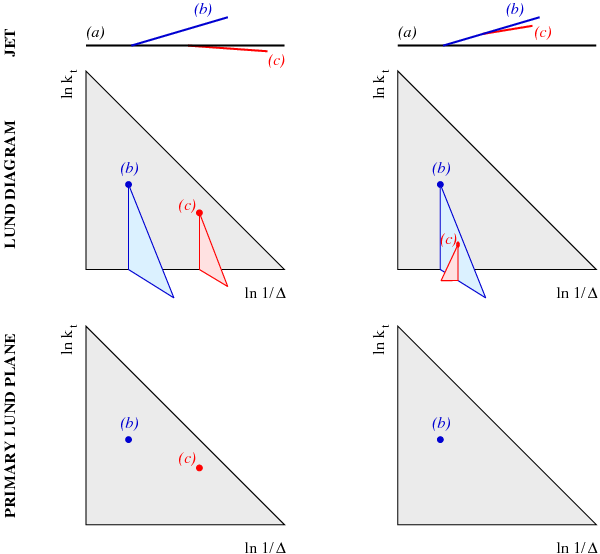
\includegraphics[width=1.0\textwidth]{visuals/figs_lund.png}
\caption{The primary and secondary lund planes for 2 example jets~\cite{Dreyer:2018nbf}.}
\label{fig:lund}
\end{figure}


$P_q(z,\theta^2) dz d \theta^2 = \frac{\alpha_s C_F}{\pi} d( log\frac{1}{z}  ) d(log \frac{1}{ \theta^2})  $\newline

Jets can also be initiated by gluons and this probability is incredibly similar :


$P_q(z,\theta^2) dz d \theta^2 = \frac{\alpha_s C_A}{\pi} d( log\frac{1}{z}  ) d(log \frac{1}{ \theta^2})  $\newline


This similarity allows us to interpret the variations in quark enriched and gluon enriched jet samples in terms of the fundamental $C_F$ and adjoint $C_A$ casimirs, in $SU(3)$ ,   $C_F = \frac{4}{3}$ and $C_A=3$. 


Comparing the probability of a quark to emit a gluon and that of a gluon to to emit a gluon, we can see the ratio is simply $\frac{C_A}{C_F} =\frac{9}{4} $. This has strong experimental implications since it implies gluon jets will on average be composed of about twice as many constituent particles as quark jets.

\chapter{Jets in Proton-Proton Collisions}%\label{ch1:intro}

A jet is a collimated grouping of hadrons usually associated with the production of a parton, quark or gluon, in this case initiated by the hard scatter of 2 constituent partons from protons. The initial parton radiates other quarks and gluons, called the "Parton Shower" and either way all color charged particles fragment into hardons, mainly pions and kaons,  before reaching the detector. Studies of jets at LHC are complicated by experimental complexities such as "underlying event", other partons from the same proton iteracting and depoiting energy in the same region of the detector. "Pileup" is also increasingly relevant, like "underlying event" but initiated from other proton interactions from this or a previous bunch since LHC collides $~10^{11}$ protons in bunches every 25 nanoseconds. Lastly any measurement is limited by the resolution of the measurement device and any detector effects which are disentangled from the signal by "unfolding" the reconstructed distributions back to generator level.

While jets are often used as simple proxies for the quark or gluon from which they originated, the structure of the radiation pattern of the hard scatter is encoded within the jet's constituent particles~\cite{Asquith:2018igt}. Jet studies are essential for a complete understanding of proton-proton interactions since the majority of interesting physics signatures contain a color charged parton in the final state. This chapter covers the basics of jet physics at LHC, from the algorithms used for clustering the constituent particles in experimental data to the language and calculations of the theory.

% cite https://arxiv.org/pdf/1901.10342.pdf simones book



\section{Jet Clustering Algorithms}\label{secSM:ch1}





sequential recombination algorithms
%# https://arxiv.org/pdf/1304.1025.pdf
%Sequential recombination algorithm for jet clustering and
KT - > C/A -> Anti-KT
\cite{Tseng:2013dva}



%##image C/A vs anti-Kt --- visuals/config-antikt-double-lund
\begin{figure}[htb]
\centering
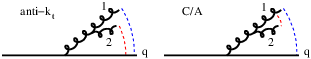
\includegraphics[width=1.0\textwidth]{visuals/config-antikt-double-lund.png}
\caption{How clustering follows radiation pattern for different algorithms~\cite{Dreyer:2018nbf}.}
\label{fig:lund}
\end{figure}

\begin{figure}[htb]
\centering
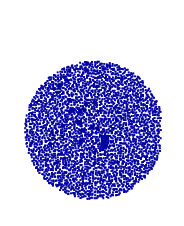
\includegraphics[width=1.0\textwidth]{visuals/figs_subjet-plots-antikt.png}
\caption{How clustering looks for Anti-Kt, circular pattern makes pileup and underlying event subtraction more simple for experimentalists~\cite{Dreyer:2018nbf}.}
\label{fig:lund}
\end{figure}

\begin{figure}[htb]
\centering
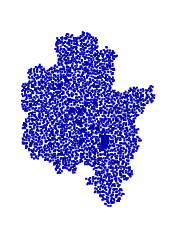
\includegraphics[width=1.0\textwidth]{visuals/figs_subjet-plots-CA.png}
\caption{C/A, not circular, shaped like radiation pattern~\cite{Dreyer:2018nbf}.}
\label{fig:lund}
\end{figure}
%#

%#


\section{Jet Structure}\label{jetstruc:ch1}

The picture is not so simple, we have pileup and underlying event. We analyze the entire radiation pattern and from its structure can determine the probability that a  gluon or quark (even the type of quark) initiated this jet there exist many methods for going about these tasks.

Quark/Gluon discrimination is discussed in section QUARK GLUON SECTION and can be done in many ways such as examining the gluon emission spectrum as visualized in the lund plane as mentioned in the introduction. In this section quark jet discrimination is discussed, specifically how the higher order corrections to the hard process are nessessary in order to properly predict measurements in the non-perturbative regime.

NLO + NLL + NP to match data in non-perturbative regime

\begin{figure}[htb]
\centering
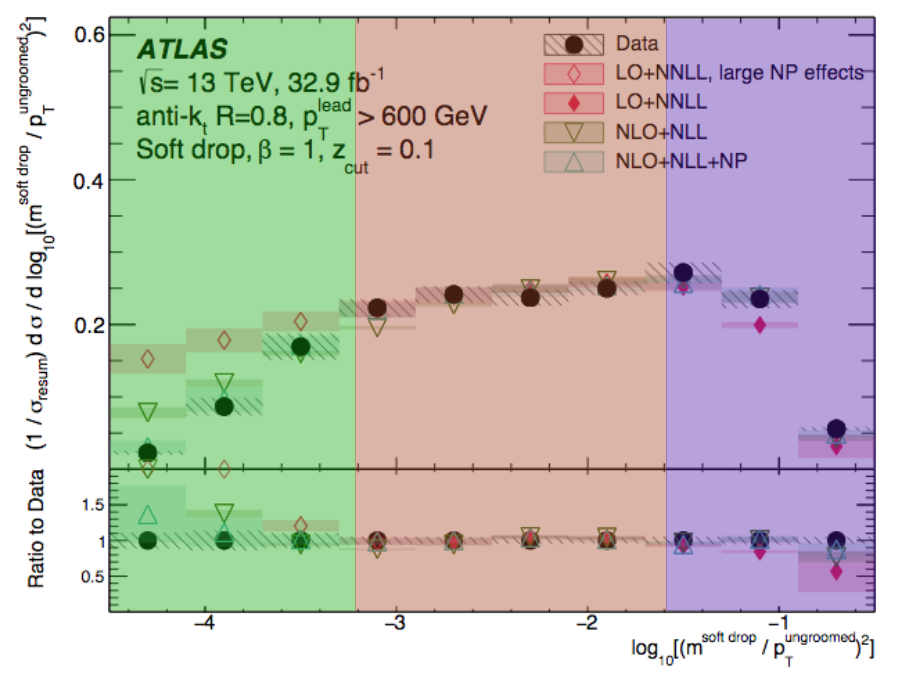
\includegraphics[width=1.0\textwidth]{visuals/ATLAS-rho-highorder.png}
\caption{ATLS DIJets Rho result~\cite{Dreyer:2018nbf}.}
\label{fig:lund}
\end{figure}



% pilup images with diff algorithms
%# https://arxiv.org/pdf/1304.1025.pdf
%Sequential recombination algorithm for jet clustering and

%Towards Jetography
%Gavin P. Salam
%$https://arxiv.org/abs/0906.1833
\cite{Salam:2009jx}

\cite{Asquith:2018igt}
%https://arxiv.org/pdf/1803.06991.pdf
%Jet Substructure at the Large HadronCollider :  Experimental Review

\section{Jet Grooming}\label{jetgroom:ch1}

Soft-drop

other grooomers

image of soft drop compared to others

image of soft drop grooming tree


%Casimir Meets Poisson: Improved Quark/Gluon Discrimination with Counting Observables
%https://arxiv.org/abs/1704.06266
%soft drop multiplicity


%%%%%%%%%%%%%%%%%%%%%%%%%%%%%%%%%%%%%%%%%%%%%%%%%%%%%%


\section{Soft-Collinear Effective Theory}\label{sec:SCET}
%https://arxiv.org/pdf/1410.1892.pdf


Below the factorization structure of the double differential jet production cross section is displayed in the context of Soft-Collinear Effective Theory, SCET, following the framework for inclusive jet production $pp \rightarrow jet + X$ developed in for jets of  %https://arxiv.org/abs/1801.00790

\begin{equation}
\frac{d \sigma}{ d p_{T} d m}=\sum_{a b c} f_{a}\left(x_{a}, \mu\right) \otimes f_{b}\left(x_{b}, \mu\right) \otimes H_{a b}^{c}\left(x_{a}, x_{b}, p_{T} / z, \mu\right) \otimes \mathcal{G}_{c}\left(z, p_{T} R, m, \mu, z_{\mathrm{cut}}, \beta\right)
\end{equation}
% equation from here https://arxiv.org/pdf/1811.06983.pdf

Jet and Soft Functions 


Image of factorization in this context

%SCET-factorization
~\cite{Becher:2014oda}
%https://arxiv.org/abs/1410.1892
\begin{figure}[htb]
\centering
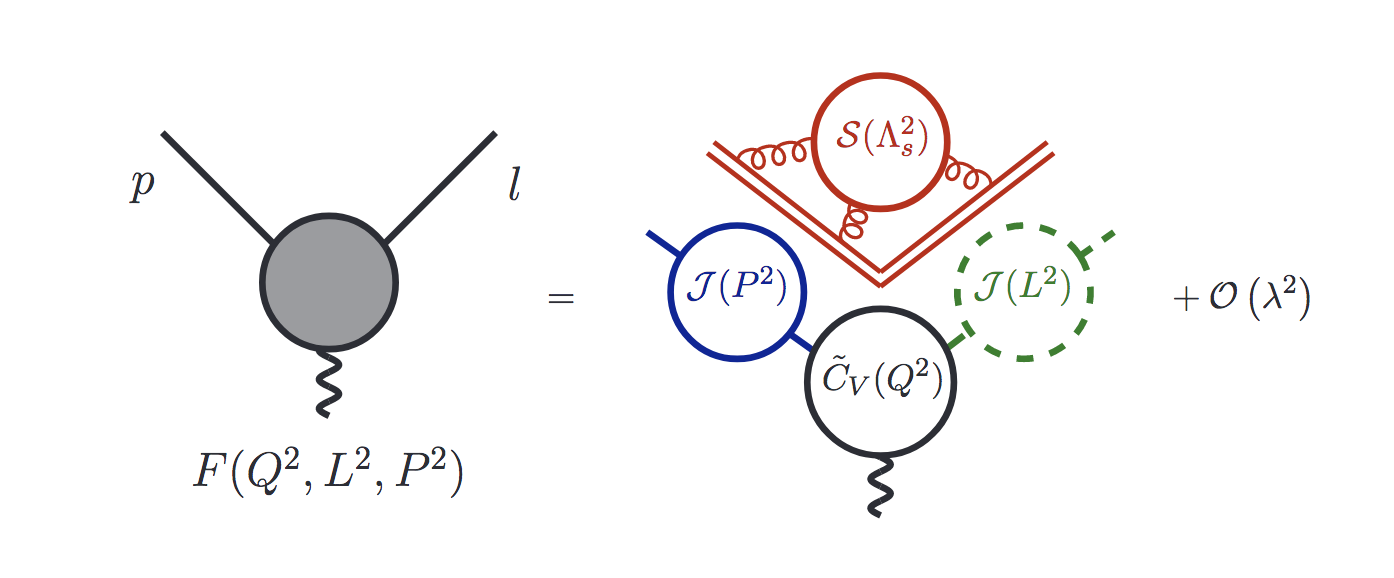
\includegraphics[width=1.0\textwidth]{visuals/SCET-factorization.png}
\caption{Fatorization of the energy scales in a hard scatter interaction according to SCET ~\cite{Becher:2014oda}.}
\label{fig:scet}
\end{figure}
discuss groomed jets in this context

comparing groomed  (Jet) to ungroomed (Jet+Soft)


%%%%%%%%%%%%%%%%%%%%%%%%%%%%%%%%%%%%%%%%%%%%%%%%%%%%%%%%%%%%%%%%%%%%%%%%%%%%%%%%%%%%%%%%%%%%%%

\section{Jets Initited by Quarks and Gluons }\label{sec:quarkandgluonjets}



%earlier discussed $C_F = \frac{4}{3}$ and $C_A=3$ 

%CITE A Theory of Quark vs. Gluon Discrimination
% https://arxiv.org/pdf/1906.01639.pdf

%Dijets make quark gluon admixture %cite SMP-16-10
%Z+Jets make mostly light quark jets, studied here and in 7 TeV analysis (1 D unfolding there and no soft drop)

% http://cms-results.web.cern.ch/cms-results/public-results/publications/SMP-16-010/index.html




% ATLAS thesis http://inspirehep.net/record/1672323/files/2016_Mantifel_PhD_Atlas_Z.pdf

In order to emphasize the relevance to the measurement presented herein, the phenomenology of Quantum Chromodynamics is discussed rather than the Lagrangian perspective. This is useful as jet studies help probe QCD in the soft and collinear limits. 
% https://arxiv.org/pdf/1709.06195.pdf CITE THIS LECTURE
Jets are formed by the hadronization of quarks and gluons. In this thesis I present a measurement of a light quark enriched jet sample. 



Consider the simplest process that could produce a quark initiated jet, a quark of energy $E_q$  emitting a gluon of energy $E_g$. The probability that this will occur is a function of the gluon's energy fraction, $z$, and the emission angle , $\theta$  \cite{Larkoski:2017fip}.\newline


$z = \frac{E_g}{E_q + E_g}$\newline

$1 - cos \theta = \frac{m^2}{2 E_q E_g}$\newline

Then the probability of gluon emission from the quark is :


$P_q(z,cos \theta) dz d cos \theta = \frac{\alpha_s C_F}{\pi}  \frac{dz}{z} \frac{dcos \theta}{1 - cos \theta}  $\newline

It is useful to assume the small angle approximation, $\theta << 1$, giving:\newline


$P_q(z,\theta^2) dz d \theta^2 = \frac{\alpha_s C_F}{\pi}  \frac{dz}{z} \frac{d \theta^2}{ \theta^2}  $\newline

Notice that the probability of emission diverges for very soft (small z) or very collinear (small $\theta$) gluons. In the soft and collinear limits the probability can be interpretted as an expectation value for the number of soft/collinear gluons \cite{Larkoski:2017fip}.

It is elucidating to rewite the probability in terms of inverse logarithms in the and introduce the "Lund Diagram" in order to visualize the uniform distribution of soft and collinear gluons in the $log \frac{1}{ \theta^2} , log\frac{1}{z} $ space.

\begin{figure}[htb]
\label{fig:lund}
\centering
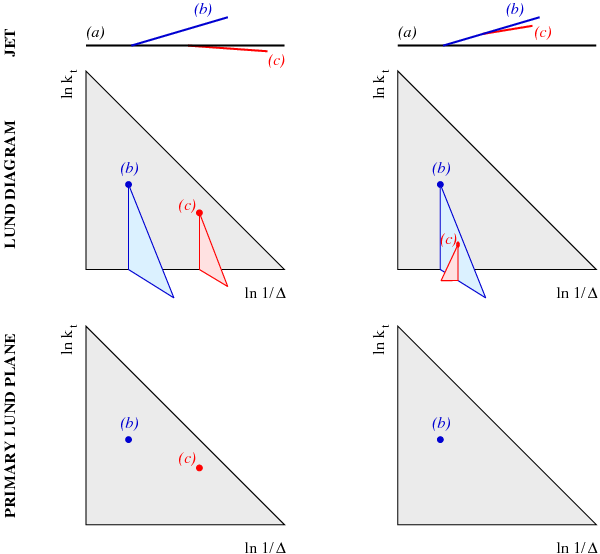
\includegraphics[width=1.0\textwidth]{visuals/figs_lund.png}
\caption{The primary and secondary lund planes for 2 example jets~\cite{Dreyer:2018nbf}.}

\end{figure}


The primary lund plane is shown in Figure ~/ref{fig:lund} ~\cite{Dreyer:2018nbf}
%image 



$P_q(z,\theta^2) dz d \theta^2 = \frac{\alpha_s C_F}{\pi} d( log\frac{1}{z}  ) d(log \frac{1}{ \theta^2})  $\newline

At leading order (LO) jets can also be "initiated" by gluons and this probability is incredibly similar :


$P_q(z,\theta^2) dz d \theta^2 = \frac{\alpha_s C_A}{\pi} d( log\frac{1}{z}  ) d(log \frac{1}{ \theta^2})  $\newline


This similarity allows us to interpret the variations in quark enriched and gluon enriched jet samples in terms of the fundamental $C_F$ and adjoint $C_A$ casimirs, in $SU(3)$ ,   $C_F = \frac{4}{3}$ and $C_A=3$. This is also the only difference between quark and gluon jet masses at LO as shown in ~\ref{sec:jetmass}.


Comparing the probability of a quark to emit a gluon and that of a gluon to to emit a gluon, we can see the ratio is simply $\frac{C_A}{C_F} =\frac{9}{4} $. This has strong experimental implications since it implies gluon jets will on average be composed of about twice as many constituent particles as quark jets, and will be broader. This will cause gluon jets to have higher mass, since the mass of a $1 \rightarrow 2 $ splitting is given by $\theta \simeq \frac{2}{\gamma} $, this is derived in ~\ref{chap:RelativisticKinematics},.






\chapter{CMS Experiment at LHC}\label{chap:CMS}

\vspace{-3pt}
\section{The Large Hadron Collider}\label{sec:ch2:lhc}

The LHC is the largest machine created my mankind to date and currently the world's highest energy particle accelerator, it accelerates and collides bunches of $~10^{11}$ protons at a time which collide at combined center-of-mass energy of 13 TeV.



\vspace{-3pt}
\section{The CMS Detector}\label{sec:CMSDetector}



The Compact Muon Solenoid (CMS) detector was used to collect the data presented in this thesis, it is one of two large general purpose detectors at the LHC. CMS experiment has recorded 162 $fb^{-1}$ integrated luminosity in the dataset presented in this thesis, collected during Run 2 of LHC.

CMS is one of 4 detectors that measure collisions of protons and lead ions produced by the Large Hadron Collider, LHC, at CERN. CMS is the smaller, overall length of 22m, a diameter of 15m, and weighs 14\,000 tonnes, of the 2 large general-purpose detectors, the other being ATLAS. The most notable feature of the detector is it's powerful 3.8 Tesla solenoid magnet, the largest superconducting magnet ever built, as of the year 2011.


The central feature of the CMS apparatus is a superconducting solenoid of 6 m internal diameter, providing a magnetic field of 3.8 T. Within the solenoid volume are a silicon pixel and strip tracker, a lead tungstate crystal electromagnetic calorimeter, and a brass and scintillator hadron calorimeter, each composed of a barrel and two endcap sections. Forward calorimeters, made of steel and quartz-fibres, extend the pseudorapidity coverage provided by the barrel and endcap detectors. Muons are detected in gas-ionization chambers embedded in the steel flux-return yoke outside the solenoid. 


%https://twiki.cern.ch/twiki/bin/viewauth/CMS/Internal/PubDetector

\subsection{Calorimeter Energy Resolution}\label{sec:CMSDetectorCalo}

 In the barrel section of the ECAL, an energy resolution of about 1\% is achieved for unconverted or late-converting photons that have energies in the range of tens of GeV. The remaining barrel photons have a resolution of about 1.3\% up to a pseudorapidity of $\abs{\eta} = 1$, rising to about 2.5\% at $\abs{\eta} = 1.4$. In the endcaps, the resolution of unconverted or late-converting photons is about 2.5\%, while the remaining endcap photons have a resolution between 3 and 4\%~\cite{CMS:EGM-14-001}.The lead tungstate crystals are $25.8 X_0$ thick in the barrel and $24.7 X_0$ thick in the endcaps. When combining information from the entire detector, the jet energy resolution amounts typically to 15\% at 10\GeV, 8\% at 100\GeV, and 4\% at 1\TeV, to be compared to about 40\%, 12\%, and 5\% obtained when the ECAL and HCAL calorimeters alone are used.

 \section{From Calorimeter Energy Deposits to Jets}\label{sec:CMSDetectorJets}

In the region $\abs{\eta} < 1.74$, the HCAL cells have widths of 0.087 in pseudorapidity and 0.087 in azimuth ($\phi$). In the $\eta$-$\phi$ plane, and for $\abs{\eta} < 1.48$, the HCAL cells map on to $5 \times 5$ arrays of ECAL crystals to form calorimeter towers projecting radially outwards from close to the nominal interaction point. For $\abs{ eta }$ > 1.74, the coverage of the towers increases progressively to a maximum of 0.174 in $\Delta \eta$ and $\Delta \phi$. Within each tower, the energy deposits in ECAL and HCAL cells are summed to define the calorimeter tower energies, subsequently used to provide the energies and directions of hadronic jets.

Jets are reconstructed offline from the energy deposits in the calorimeter towers, clustered using the anti-\kt algorithm~\cite{Cacciari:2008gp, Cacciari:2011ma} with a distance parameter of 0.4. In this process, the contribution from each calorimeter tower is assigned a momentum, the absolute value and the direction of which are given by the energy measured in the tower, and the coordinates of the tower. The raw jet energy is obtained from the sum of the tower energies, and the raw jet momentum by the vectorial sum of the tower momenta, which results in a nonzero jet mass. The raw jet energies are then corrected to establish a relative uniform response of the calorimeter in $\eta$ and a calibrated absolute response in transverse momentum \pt. 


 \section{Muon Reconstruction}\label{sec:CMSDetectorMuons}


Muons are measured in the pseudorapidity range $\abs{\eta} < 2.4$, with detection planes made using three technologies: drift tubes, cathode strip chambers, and resistive plate chambers. The single muon trigger efficiency exceeds 90\% over the full $\eta$ range, and the efficiency to reconstruct and identify muons is greater than 96\%. Matching muons to tracks measured in the silicon tracker results in a relative transverse momentum resolution, for muons with \pt up to 100\GeV, of 1\% in the barrel and 3\% in the endcaps. The \pt resolution in the barrel is better than 7\% for muons with \pt up to 1\TeV~\cite{Sirunyan:2018fpa}. 


A more detailed description of the CMS detector, together with a definition of the coordinate system used and the relevant kinematic variables, can be found in Ref.~\cite{Chatrchyan:2008zzk}.  The global event reconstruction (also called particle-flow event reconstruction~\cite{CMS-PRF-14-001}) is described in ~\ref{sec:PFReco}.




% riju https://adasgupt.web.cern.ch/adasgupt/locked/thesis.pdf
\chapter{Measurement of the differential jet production cross section with respect to jet mass and transverse momentum in
Z + Jet events from pp collisions at $\sqrt{s}$ = 13 TeV}\label{chap:AN-18-240}

% copied from AN-18-240.tex

%\input{/Users/Om/Documents/thesis/AN-18-240/AN-18-240.tex}


Abstract.

We present a measurement of the differential jet production cross
section as a function of the jet mass and transverse momentum in
events with a Z + Jet topology, with and without a jet grooming
algorithm applied. For ungroomed jets, leading-order and next-to-leading order
QCD Monte Carlo programs are found to predict the jet mass
spectrum in the data reasonably well, with some disagreement
at very low and very high masses. 
For groomed jets, the agreement between the Monte Carlo programs and the data
improves overall, and extends lower in jet mass due to the removal of soft and
collinear portions of the jet. 
First-principles theoretical calculations of the groomed jet mass are in preparation by theorists to be compared
to the data. 




%%%
%%% INTRO
%%%


\section{Introduction}

\input{AN-18-240/introduction.tex}

%%%
%%%  DATA and MC 
%%%
\section{Data and MC}

\input{AN-18-240/dataandmc.tex}



%%%
%%%             TRIGGER
%%%
\section{Trigger}

The data are collected with single-lepton triggers, with muons (electrons) of $pt > 29 (37)$ GeV using the $IsoMu27$ ($Ele35_WPTight_Gsf$ $ || $ $ Photon200 $) triggers, as recommended by the muon (egamma) POG. All triggers used for this analysis are prescaled to 1. 




%%%
%%%                        RECO and SELECTION
%%%

\section{Reconstruction and Selection}


\input{AN-18-240/recoandsel.tex}

\section{Data to MC Comparisons}


\input{AN-18-240/datatomccomp.tex}




\section{Detector Response}

\input{AN-18-240/detresp.tex}



%%%%%%%%%%%


% MASS RESPONSE MATRICES

\input{AN-18-240/responsematrix_u.tex}


\input{AN-18-240/responsematrix_sdB0.tex}

% RHO RESPONSE MATRICES
\input{AN-18-240/rhoresponsematrix_u.tex}


\input{AN-18-240/rhoresponsematrix_sdB0.tex}


%PURITY and STABILITY

\input{AN-18-240/purity_u.tex}

\input{AN-18-240/purity_sdB0.tex}




\section{Uncertainties}

\input{AN-18-240/uncert.tex}


\section{Unfolding}

\input{AN-18-240/tunfolding.tex}

\section{Results}

\input{AN-18-240/results.tex}

\section{Summary}

In conclusion, we have presented a differential jet cross section measured in Z + Jet events in
bins of the ungroomed jet $\pt$ in conjunction with the ungroomed and groomed
jet mass (as well as dimensionless mass) using the ``soft drop'' (a.k.a. ``modified mass drop
tagger'') algorithm with 9 different combinations of parameters. 
The results are presented as the normalized cross section, normalized per reconstructed jet $\pt$ bin. 
Overall leading-order MC simulation agrees
reasonably well with the data within our uncertainties. 
Agreement below the Sudakov peak is slightly
worse than above. The application of a grooming algorithm
improves the overall precision, with larger improvement at low jet masses. 
This analysis improves over previous iterations by using various parameter values for the ``soft drop''
jet grooming algorithm, as well as by including an additional unfolding in both transverse momentum
and dimensionless mass, as was done by the ATLAS collaboration \cite{Aaboud:2017qwh} .





\appendix

\section{2016 data results}

This Appendix shows the distributions from the "Detector Response" through the "Results" sections of the main analysis note with only the 2016 data rather than the full Run 2 statistics seen in the main body of the note.



% MASS RESPONSE MATRICES

../../AN-18-240/responsematrix_u_2016.tex


../../AN-18-240/responsematrix_sdB0_2016.tex

% RHO RESPONSE MATRICES
%\input{rhoresponsematrix_u_2016.tex}


%\input{rhoresponsematrix_sdB0_2016.tex}


%PURITY and STABILITY

../../../AN-18-240/purity_u_2016.tex

../../../AN-18-240/purity_sdB0_2016.tex



../../../AN-18-240/uncert_2016.tex


../../../AN-18-240/tunfolding_2016.tex



../../../AN-18-240/results_2016.tex



%\section{Data and MC comparisons for soft-dropped jet masses}
\section{2017 data results}

This Appendix shows the distributions from the "Detector Response" through the "Results" sections of the main analysis note with only the 2017 data rather than the full Run 2 statistics seen in the main body of the note.



% MASS RESPONSE MATRICES

../../AN-18-240/responsematrix_u_2017.tex


../../AN-18-240/responsematrix_sdB0_2017.tex

% RHO RESPONSE MATRICES
%\input{rhoresponsematrix_u.tex}


%\input{rhoresponsematrix_sdB0.tex}


%PURITY and STABILITY

../../AN-18-240/purity_u_2017.tex

../../AN-18-240/purity_sdB0_2017.tex



../../AN-18-240/uncert_2017.tex


../../../AN-18-240/tunfolding_2017.tex



../../AN-18-240/results_2017.tex




\section{2018 data results}

This Appendix shows the distributions from the "Detector Response" through the "Results" sections of the main analysis note with only the 2018 data rather than the full Run 2 statistics seen in the main body of the note.



% MASS RESPONSE MATRICES

../../AN-18-240/responsematrix_u_2018.tex


../../AN-18-240/responsematrix_sdB0_2018.tex

% RHO RESPONSE MATRICES
%\input{rhoresponsematrix_u_2016.tex}


%\input{rhoresponsematrix_sdB0_2016.tex}


%PURITY and STABILITY

../../AN-18-240/purity_u_2018.tex

../../../AN-18-240/purity_sdB0_2018.tex



../../../AN-18-240/uncert_2018.tex


../../../AN-18-240/tunfolding_2018.tex



../../AN-18-240/results_2018.tex





\chapter{Identification and Calibration of Boosted Hadronic W
Bosons within Fully Merged Top Quark Jets at 13 TeV}\label{chap:AN-17-177}

\chapter{Conclusion}\label{chap:conclusion}

\vspace{-5pt}
\section{Conclusion}\label{sec:concld}


The measurement matches the theoretical calculations well, i hope.


\center{The End.}

%%%%%%%%%%%%%%%%%%%%%%%%%%%%%%%%%%%%%%%%%%%%%%%%%%%%%%%%%%%%%%
% Appendices
%
% Because of a quirk in LaTeX (see p. 48 of The LaTeX
% Companion, 2e), you cannot use \include along with
% \addtocontents if you want things to appear the proper
% sequence. Since the PSU Grad School requires
%%%%%%%%%%%%%%%%%%%%%%%%%%%%%%%%%%%%%%%%%%%%%%%%%%%%%%%%%%%%%%%
%\appendix
%

\chapter{Relativistic Kinematics}\label{chap:RelativisticKinematics}


\begin{figure}[htb]

\centering
\includegraphics[width=1.0\textwidth]{visuals/1to2splitting.png}
\caption{ A simple $ 1 \rightarrow 2  $ decay described by relativistic kinematics.}
\label{onetotwo}
\end{figure}

Consider the LO process depicted in ~\ref{onetotwo}, of a simple $ 1 \rightarrow 2  $ decay.


at LO there is a kinematic turn-off at $\pt R/2$ (where $R$ is the
distance parameter for the jet clustering), from the relativistic kinematics of a $1\rightarrow 2$ decay. 
However, for real jets the turn-off is closer to $\pt R/\sqrt{2}$ due to stochastic effects. 
To see this, consider a particle of energy $E$ and mass $m$ decaying to two massless
particles, each with an energy $E/2$ and separated by an angle $\theta$. 
The mass must satisfy $m^2 < \frac{E^2}{2}\left( 1 - \cos{\theta}\right)$. In the small
angle limit, this would be $m^2 < E^2\theta^2/4$, or $m < E\theta/2$.





According to relativistic kinematics the interaction can be described by the following equation:\newline

$p^{\mu} p_{\mu}  =  (p_1 + p_2)^{\mu} (p_1 + p_2)_{\mu}  $\newline

$p^{\mu} p_{\mu}  =  (p_1 + p_2)^{\mu} (p_1 + p_2)_{\mu}  $\newline

$m^2  = (E_1 + E_2)^2  - (\vec{p_1} + \vec{p_2} ) \dot (\vec{p_1} + \vec{p_2} )  $\newline


$m^2  \simeq 2 E_1 E_2 (1 - \cos \theta ) $\newline

If the energies of the splitting particles are equal then the equation simplifies since  $ E_1 = E_2 = \frac{E}{2} $ .


$m^2  < \frac{E^2}{2} ( 1 - \cos{\theta}  $\newline

$\frac{2m^2}{E^2}  < ( 1 - \cos{\theta}  $\newline

Using the small angle approximation this simplifies further.

$(1 - (1- \frac{\theta^2}{2}) )  \simeq  \frac{\theta^2}{2}  $\newline

Solving for mass, one finds :\newline

$m < E\theta/2$\newline

With more particle decays, the stochastic nature of the shower increases this to $m < E\theta/\sqrt{2}$.
Thus, a leading-order ($1\rightarrow 2$) decay will have a faster kinematic
turn-off than an all-orders ($1 \rightarrow$ many) decay.\newline

Solving for theta:\newline
 $\theta < \frac{2}{\gamma}$ where $\gamma$ is the lorentz factor $\gamma = \frac{1}{\sqrt{1-\frac{v^2}{c^2}}}  $.
%\chapter{Introduction}\label{chap:intro}

% \vspace{-5pt}
\section{Motivation}\label{sec:ch1:intro}

Within this dissertation, I provide a measurement of the differential jet cross section, as a function of the jet mass and transverse momentum, in events with a Z + Jet topology, with and without a jet grooming algorithm applied, using data collected by CMS experiment at LHC. The jet grooming used was the ``Soft Drop''
procedure 
%~\cite{softdrop}, wuth multiple values of the tunable parameters $\beta$ and $z_{cut}$. This represents the first, to my knowledge, measurement of it's kind with a light quark enriched jet sample at $\sqrt{s}$ = 13 TeV. 

Softdrop iteratively declusters a jet $j$ with distance parameter $R$ into two subjets, $j_1$ and $j_2$.
If the softdrop condition

\begin{equation}
  \frac{\min(p_{T1},p_{T2})}{p_{T1}+p_{T2}} > z_{cut} \cdot (\frac{\Delta R_{12}}{R})^\beta
\end{equation}

is met, then the procedure stops and $j$ is the final jet. Otherwise, the declustering continues - 
the higher $pt$ subjet is relabeled as $j$ and the lower $pt$ one is dropped.
By design, this condition fails for wide-angle soft radiation, which is therefore removed by the soft
drop procedure. The tunable parameters, $\beta$ and $z_{cut}$, control the degree of jet grooming:
$\beta$ tunes the algorithm's sensitivity to wide-angle radiation, while $z_{cut}$ sets the energy scale
of the grooming. In the case of $\beta \rightarrow \infty$, an ungroomed jet is returned. 
In the $\beta = 0$ case, the soft drop procedure is identical to the ``modified mass drop tagger'' (MMDT)
from Ref.
%~\cite{mmdt}. The soft drop algorithm removes soft and wide-angle radiation
from jets in a very theoretically controlled manner, making it suitable to separate
the ``hard'' and ``soft'' parts of the jet. Specifically, the soft drop
algorithm can remove non-global logarithms from correlations of
radiation within and between jets, which are extremely difficult to
compute theoretically
%~\cite{Dasgupta:2001sh,mmdt,softdrop,Dasgupta:2013via,Dasgupta:2015yua,Larkoski:2015zka}.

Comparing the production cross section for groomed and ungroomed jets separately allows us to
gain sensitivity to both the ``hard'' and ``soft'' jet physics. 
The groomed cross section can be directly compared to theoretical calculations of the jet mass
now and in the future, which is a very active area of theoretical research
at this time
%~\cite{Dasgupta:2012hg,Chien:2012ur,Jouttenus:2013hs,Almeida:2014uva,Liu:2014oog,Stewart:2014nna,Khelifa-Kerfa:2015mma,Frye:2016aiz,Kolodrubetz:2016dzb}. Furthermore, separating the hard and soft jet physics
allows a deeper understanding of the various effects involved in QCD
%radiation. In particular, Ref.~\cite{Frye:2016aiz} calculates the
groomed jet mass at next-to-next-to-leading order using soft colinear effective theory, matched to a
%parton shower at leading order using {\tt MCFM}~\cite{MCFM1,MCFM2}, and the authors of Ref.~\cite{mmdt} have
provided a next-to-leading logarithm calculation with traditional perturbative QCD, matched to a 
parton shower at leading order, also using {tt MCFM}.  We compare these theoretical predictions 
to our data in this paper for the first time in this channel at CMS. Both CMS and ATLAS have similar measurements in a dijet sample at %Ref.~\cite{cms_jetmassDijet, atlas_jetmass2}.

The analysis strategy is similar to that of %Ref.~\cite{cms_jetmassDijet}.
However, there are several differences. As in that paper, the cross section is also
unfolded in both jet mass and $pt$, however we also provide the measurement in jet $\rho$, dimensionless mass , and $pt$. While the previous measurement considered only one value for the soft drop parameter $\beta$, this analysis considers several.
We apply the soft drop algorithm to compare
directly to theoretical computations. Additionally, we not only measure the cross section as a function of mass, but also as a function of dimensionless mass, $\rho = 2log(m/(pt R))$, as is also done in the previously mentioned ATLAS measurement.  The dimensionless mass $\rho$ only weakly depends on $pt$, unlike mass, which is highly correlated. Additionally, the use of this variable aids in the separation of fixed order, perturbative and non-perturbative effects.
Finally, we also present the normalized differential cross section. We compute the cross sections normalized per $pt$ bin
(the ``normalized'' cross section) with respect to the jet $pt$ and jet mass 
by unfolding a binned two-dimensional distribution in $pt$ and mass
with widths $\Delta pt$ and $\Delta m$, respectively.

The normalized differential cross section in two forms :

\begin{equation}
\frac{1}{d\sigma/dpt}\frac{d^2\sigma}{dpt\,dm} = \frac{1}{N/\Delta pt} R(\frac{N_{ij}}{ \Delta pt \,\Delta m} )
\end{equation}


as well as :

\begin{equation}
\frac{1}{d\sigma/dpt}\frac{d^2\sigma}{dpt\,d\rho} = \frac{1}{N/\Delta pt} R(\frac{N_{ij}}{ \Delta pt \,\Delta \rho} )
\end{equation}


where $N$ is the total number of $Z+$jets events in our selection,
$N_{ij}$ is the number of such events in $pt$ bin $i$ and mass ($\rho$) bin $j$,
and $R(\alpha)$ is the unfolding procedure applied to the two-dimensional
distribution $\alpha$.

The 2 above normalized distributions are provided within for ungroomed  and groomed jets Anti-Kt Radious R$= 0.8$ jets. The groomed measurement is given in 9 configurations, one measurement is shown for jets groomed with every combination of 3 possible $\beta$ and $z_{cut}$ values (Where $\beta$ = 0 and $z_{cut}$ = 0 .1 is the current CMS default ):


$ \beta = [ 1,  0 , -1 ]  $

$ z_{cut}  = [ 0.15, 0.1, 0.05 ] $ 


These measurements currently represent humanity's highest energy measurement of a light quark enriched jet production cross section.


%%%%%%%%%%%%%%%%%%%%%%%%%%%%%%%%%%%%%%%%%%%%%%%%%%%%%%%%%%%%%%%
% ESM students need to include a Nontechnical Abstract as the %
% last appendix.                                              %
%%%%%%%%%%%%%%%%%%%%%%%%%%%%%%%%%%%%%%%%%%%%%%%%%%%%%%%%%%%%%%%
% This \include command should point to the file containing
% that abstract.
%\include{nontechnical-abstract}
%%%%%%%%%%%%%%%%%%%%%%%%%%%%%%%%%%%%%%%%%%%
} % End of the \allowdisplaybreak command %
%%%%%%%%%%%%%%%%%%%%%%%%%%%%%%%%%%%%%%%%%%%

%%%%%%%%%%%%%%%%
% BIBLIOGRAPHY %
%%%%%%%%%%%%%%%%
% You can use BibTeX or other bibliography facility for your
% bibliography. LaTeX's standard stuff is shown below. If you
% bibtex, then this section should look something like:
   \begin{singlespace}
   \bibliographystyle{unsrt}
   \phantomsection \addcontentsline{toc}{chapter}{Bibliography}
   \bibliography{ref}
   \end{singlespace}

%\begin{singlespace}
%\begin{thebibliography}{99}
%\addcontentsline{toc}{chapter}{Bibliography}
%\frenchspacing

%\bibitem{Wisdom87} J. Wisdom, ``Rotational Dynamics of Irregularly Shaped Natural Satellites,'' \emph{The Astronomical Journal}, Vol.~94, No.~5, 1987  pp. 1350--1360.

%\bibitem{G&H83} J. Guckenheimer and P. Holmes, \emph{Nonlinear Oscillations, Dynamical Systems, and Bifurcations of Vector Fields}, Springer-Verlag, New York, 1983.

%\end{thebibliography}
%\end{singlespace}

\backmatter

% Vita
% \vita{SupplementaryMaterial/Vita}

\end{document}

